\documentclass[a4paper,11pt]{article}
\usepackage[a4paper]{geometry}
\usepackage{hyperref}
\usepackage{longtable}
\usepackage{float}

\usepackage{tikz-uml}
\usepackage[T1]{fontenc}

\newcommand{\tikzimgEternalWebpages}{
%%%%%%%%%%%%%
%% ETERNAL WEBPAGE OVERVIEW
%%%%%%%%%%%%%
\tikzumlset{fill class=white, fill template=white, fill package=white,fill note=white} 
\begin{tikzpicture}

\begin{umlpackage}[x=0, y=0]{Tribler}

	\begin{umlpackage}[x=0, y=0]{SiteRipper}
		%%Class definitions
		\umlclass[x=3, y=6.5]{ResourceSniffer}{}{
			+ GetFile(uri)\\
			+ StartLoading(url)\\
			+ GetWebPage()\\
			+ Seed()
		}

		\umlclass[x=0, y=3]{ResourceSeeder}{}{
			+ \umlstatic{SeedWebpage(tarfile, webpage, accessdate)}
		}

		\umlclass[x=7, y=0.2]{WebPage}{}{
			+ DownloadContent()\\
			+ AddResource(uri)\\
			+ GetContent()\\
			+ SetContent(content)\\
			+ GetUrl()\\
			+ SetUrl(url)\\
			+ CreateFromFile(tarFileName)\\
			+ RemoveTempFiles(tarFileName)\\
			+ \umlstatic{GetFileName(url)}\\
			+ \umlstatic{GetResourceFileName(url)}\\
			+ \umlstatic{GetURLName(filename)}\\
			+ \umlstatic{GetTarName(url)}\\
			+ \umlstatic{GetTarFilepath(url)}\\
			+ CreateTar()\\
			+ MapResource(url)
		}

		\umlclass[x=0, y=0]{WebPageTorrentHeader}{}{
			+ CreateTorrentDef(session)\\
			+ GetSeededFile()\\
			+ GetFileFolder()
		}

		%%Associations
		\umlaggreg[mult1=1,mult2=1,pos2=0.7]{ResourceSniffer}{WebPage} 
		\umluniassoc{ResourceSniffer}{ResourceSeeder}
		\umluniassoc{ResourceSeeder}{WebPageTorrentHeader}
	\end{umlpackage}

\end{umlpackage}

\end{tikzpicture}
}
\documentclass[tikz]{standalone}
\usepackage{tikz-uml}
\usepackage[T1]{fontenc}

\newcommand{\pckgsep}{/ } 

\begin{document}

%%%%%%%%%%%%%
%% GENERAL TUPT OVERVIEW
%%%%%%%%%%%%%
\tikzumlset{fill class=white, fill template=white, fill package=white,fill note=white} 
\begin{tikzpicture}

\begin{umlpackage}[x=0, y=0]{Tribler}

	\begin{umlpackage}[x=6, y=9]{PluginManager }
		\umlemptyclass{PluginManager}
	\end{umlpackage}

	\begin{umlpackage}[x=0, y=0]{TUPT}
		%%Class definitions
		\umlemptyclass[x=1, y=4]{Movie}
		\umlemptyclass[x=6, y=2]{TUPTControl}

		\umlemptyclass[x=1, y=2]{MovieTorrentIterator}
		\umlemptyclass[x=1, y=0]{MovieTorrent}
		\umlemptyclass[x=6, y=0]{TorrentInfoBar}

		\umlemptypackage[x=10, y=2]{Channels}
		\umlemptypackage[x=3, y=6]{Matcher}
		\umlemptypackage[x=6, y=6]{Parser}
		\umlemptypackage[x=9, y=6]{TorrentFinder}

		%%Associations
		\umluniassoc[mult1=1,mult2=1]{TUPTControl}{MovieTorrentIterator} 
		\umlcompo[mult1=1,mult2=*]{MovieTorrentIterator}{MovieTorrent}
		\umlaggreg[mult1=1,mult2=*]{MovieTorrentIterator}{Movie} 
		\umlcompo[mult1=1,mult2=1]{TUPTControl}{TorrentInfoBar}

		\umluniassoc{TUPTControl}{Channels} 
		\umluniassoc{TUPTControl}{Matcher} 
		\umluniassoc{TUPTControl}{Parser} 
		\umluniassoc{TUPTControl}{TorrentFinder} 

		\umluniassoc{Matcher}{PluginManager}
		\umluniassoc{Parser}{PluginManager}
		\umluniassoc{TorrentFinder}{PluginManager}

	\end{umlpackage}

\end{umlpackage}

\end{tikzpicture}

%%%%%%%%%%%%%
%% CHANNELS OVERVIEW
%%%%%%%%%%%%%

\tikzumlset{fill class=white, fill template=white, fill package=white,fill note=white} 
\begin{tikzpicture}

\begin{umlpackage}[x=0, y=0]{Channels}
	%%Class definitions
	\umlclass[x=0, y=0]{MovieInserter}{}{
		+ PrettyMovieName(movie, isHD)\\
		+ AddTorrentToChannel(channelId, torrentDef, name)\\
		+ ResolveTorrentConflict(channelId, torrentDef, otherInfoHash)\\
		+ Insert(torrentDef, movie, isHD)\\
		+ InsertThreaded(torrentDef, movie, isHD)()
	}

	\umlclass[x=11, y=0]{MovieChannelControl}{}{
		+ initAuto()\\
		+ initWithChannelSearchManager(manager)\\
		+ GetChannelNameForYear(year)\\
		+ GetChannelDescriptionForYear(year)\\
		+ GetChannelIDForYear(year)\\
		+ RemoveChannelByYear(year)\\
		+ RemoveChannelById(channelId)\\
		+ GetKnownTUPTChannels()\\
		+ GetKnownYears()\\
		+ GetChannelObjectFromID(channelID)\\
		+ UpVoteChannel(channelID)\\
		+ AddTorrentToChannel(channelID, torrentDef)\\
		+ ChannelHasTorrent(channelID, torrentDef)\\
		+ ChannelGetTorrentFromName(channelID, name)\\
		+ RemoveTorrentFromChannel(channelID, torrentDef)\\
		+ RenameChannelTorrent(channelID, torrentDef, name)
	}

	%%Associations
	\umlaggreg[mult1=1,mult2=1]{MovieInserter}{MovieChannelControl} 
\end{umlpackage}

\end{tikzpicture}

%%%%%%%%%%%%%
%% MATCHER OVERVIEW
%%%%%%%%%%%%%

\tikzumlset{fill class=white, fill template=white, fill package=white,fill note=white} 
\begin{tikzpicture}

\begin{umlpackage}[x=0, y=0]{Matcher}
	%%Class definitions
	\umlclass[x=0, y=3]{MatcherControl}{}{
		+ CorrectMovie(movie)
	}

	\umlclass[x=6, y=3,type=interface]{IMatcherPlugin}{}{
		+ MatchMovie(movie)\\
		+ GetMovieAttributes()\\
		+ GetAttribute(attribute)
	}

	\umlclass[x=6, y=0]{TheMovieDBMatcherPlugin}{}{

	}

	%%Associations
	\umlreal{TheMovieDBMatcherPlugin}{IMatcherPlugin}
	\umlaggreg[mult1=1,mult2=*]{MatcherControl}{IMatcherPlugin}
	
\end{umlpackage}

\end{tikzpicture}

%%%%%%%%%%%%%
%% PARSER OVERVIEW
%%%%%%%%%%%%%

\tikzumlset{fill class=white, fill template=white, fill package=white,fill note=white} 
\begin{tikzpicture}

\begin{umlpackage}[x=0, y=0]{Parser}
	%%Class definitions
	\umlclass[x=0, y=6]{ParserControl}{}{
		+ HasParser(url)\\
		+ ParseWebsite(url, html)
	}

	\umlclass[x=6, y=6,type=interface]{IParserPlugin}{}{
		+ ParseWebSite(url, html)\\
		+ GetParseableSites()
	}

	\umlclass[x=6, y=3]{IMDbParserPlugin}{}{

	}

	\umlclass[x=0, y=0]{NoParserFoundException}{}{

	}

	\umlclass[x=6, y=0]{IllegalParseResultException}{}{

	}

	%%Associations
	\umlreal{IMDbParserPlugin}{IParserPlugin}
	\umlaggreg[mult1=1,mult2=*]{ParserControl}{IParserPlugin}
	\umluniassoc{ParserControl}{NoParserFoundException} 
	\umluniassoc{ParserControl}{IllegalParseResultException} 
	
\end{umlpackage}

\end{tikzpicture}

%%%%%%%%%%%%%
%% TORRENT FINDER OVERVIEW
%%%%%%%%%%%%%

\tikzumlset{fill class=white, fill template=white, fill package=white,fill note=white} 
\begin{tikzpicture}

\begin{umlpackage}[x=0, y=0]{TorrentFinder}
	\umlclass[x=6, y=3.5,type=interface]{IMovieTorrentDef}{}{
		+ GetSeeders()\\
		+ GetLeechers()\\
		+ IsHighDef()\\
		+ GetMovieDescriptor()\\
		+ GetTorrentName()\\
		+ GetTorrentURL()\\
		+ GetTorrentProviderName()\\
	}

	\umlemptyclass[x=0, y=0]{FenopyMovieTorrentDef}
	\umlemptyclass[x=6, y=0]{KatPhMovieTorrentDef}
	\umlemptyclass[x=12, y=0]{TriblerMovieTorrentDef}

	\umlclass[x=6, y=9.5,type=interface]{ITorrentFinderPlugin}{}{
		+ GetTorrentDefsForMovie(movie)
	}

	\umlemptyclass[x=0, y=7]{FenopyTorrentFinderPlugin}
	\umlemptyclass[x=6, y=7]{KatPhTorrentFinderPlugin}
	\umlemptyclass[x=12, y=7]{TriblerTorrentFinderPlugin}

	\umlclass[x=6, y=12]{PluginThread}{}{
		+ run()
	}

	\umlemptyclass[x=11, y=12]{IllegalTorrentResultException}

	\umlclass[x=-1, y=16]{SortedTorrentList}{}{
		+ GetList()\\
		+ Insert(torrentDef, trust)\\
		+ SetUserDict(dict)
	}

	\umlclass[x=6, y=16]{TorrentFinderControl}{}{
		+ FindTorrents()\\
		+ ProcessTorrentDefList(torrentDefList, trust)\\
		+ ProcessTorrentDef(definition, trust)\\
		+ GetTorrentList()\\
		+ GetHDTorrentList()\\
		+ GetSDTorrentList()\\
		+ HasTorrent()\\
		+ HasHDTorrent()\\
		+ HasSDTorrent()\\
		+ run()\\
	}

	%%Associations
	\umlreal{FenopyMovieTorrentDef}{IMovieTorrentDef}
	\umlreal{KatPhMovieTorrentDef}{IMovieTorrentDef}
	\umlreal{TriblerMovieTorrentDef}{IMovieTorrentDef}

	\umluniassoc{FenopyTorrentFinderPlugin}{IMovieTorrentDef}
	\umluniassoc{KatPhTorrentFinderPlugin}{IMovieTorrentDef}
	\umluniassoc{TriblerTorrentFinderPlugin}{IMovieTorrentDef}

	\umlreal{FenopyTorrentFinderPlugin}{ITorrentFinderPlugin}
	\umlreal{KatPhTorrentFinderPlugin}{ITorrentFinderPlugin}
	\umlreal{TriblerTorrentFinderPlugin}{ITorrentFinderPlugin}

	\umlaggreg[mult1=1,mult2=1]{PluginThread}{ITorrentFinderPlugin}
	\umluniassoc{PluginThread}{IllegalTorrentResultException}

	\umlaggreg[mult1=1,mult2=*]{TorrentFinderControl}{PluginThread}
	\umlcompo[mult1=1,mult2=2]{TorrentFinderControl}{SortedTorrentList}

\end{umlpackage}

\end{tikzpicture}

\end{document}

\title{[P2PBrowser group] Code Architechture}
\author{Steffan Norberhuis \and Quinten Stokkink}
\date{12 June 2013}
\begin{document}
   \maketitle

\section{Introduction}
Our projects consists of two seperate extensions of Tribler. Both use wxWebview to browse the internet.
The first extension is the Eternal Webpage extension.
This extension will allow a user to easily browse the web using peer-to-peer-swarms and also add new pages to the swarm.
The second extension is the TUPT extension.
This extension allows you to browse websites and if a movie is detected on the website,
then you can begin streaming this movie with one click of a button.

The only common part between the two extensions is the WebBrowser class.
After we finished the Eternal Webpages extension, we started working on the TUPT extension.
We transformed the WebBrowser class and stripped all functionality specific for the EternalWebpages extension that was no longer needed.
All needed functionality for the TUPT extension to the WebBrowser class has been added in a generic way.
This generic approach was much harder for the WebBrowser, because we changed the way how WebBrowser loads pages.

The projects use Python 2.7 and are compiled as part of the Tribler project (see \url{https://github.com/Tribler/tribler}).
Because we cannot/should not deliver code that is not our own we have ripped out our code
from the main Tribler code. The result of this move is that the project is uncompilable and 
some of the tests unrunnable. This should not really be of any hindrance to evaluating the code though.

\section{Eternal Webpages diagrams}
The Eternal Webpages package is a Proof Of Concept package no longer undergoing 
active development. Its main purpose is to download and bundle resources referenced by a webpage
in such a way that they can be fetched offline.
To accomplish this, the webbrowser has 2 modes for viewing websites: one by browsing
the internet and one by downloading P2P cached copies of websites (called internet viewmode and
swarm viewmode respectively). This is shown in \autoref{fig:activitybrowsing}.
The package is referenced from the main Tribler projects web browser for every resource
it ecounters while loading a webpage. This is shown in \autoref{fig:activityseeding}.
The full class diagram of the package is included in \autoref{fig:classdiagrameternalweb}.

\begin{figure}[h]
  \centering
      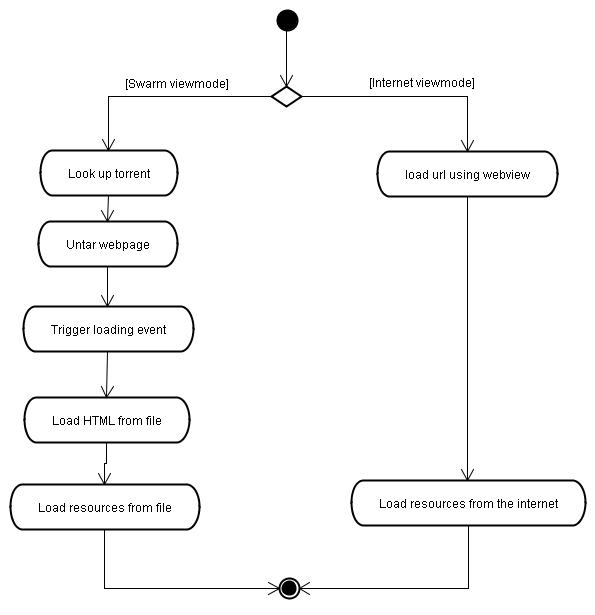
\includegraphics[width=0.8\textwidth]{SiteRipper-Browsing-activitydiagram.jpg}
  \caption{Activity diagram of viewmode based webbrowsing}
  \label{fig:activitybrowsing}
\end{figure}

\begin{figure}[h]
  \centering
      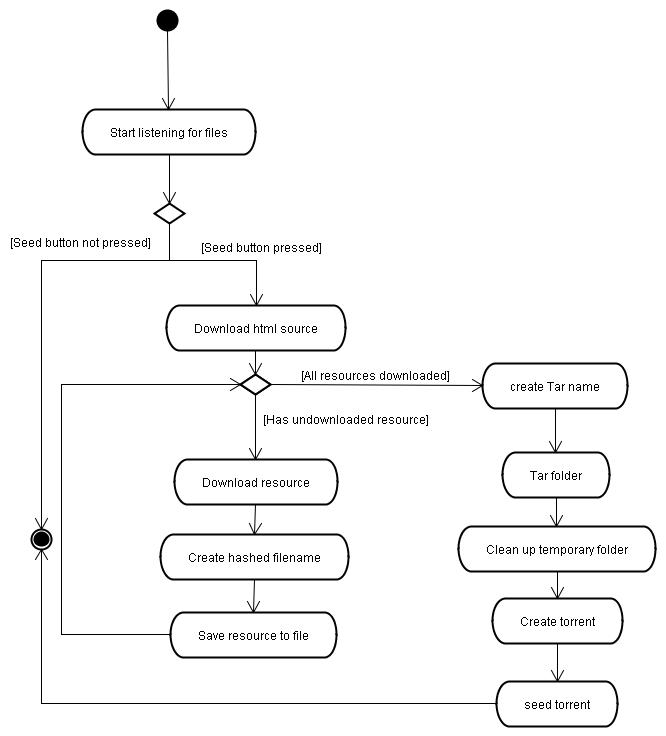
\includegraphics[width=0.8\textwidth]{SiteRipper-Seeding-activitydiagram.jpg}
  \caption{Activity diagram of seeding mode webbrowsing}
  \label{fig:activityseeding}
\end{figure}

\begin{figure}[h]
  \centering
\tikzimgEternalWebpages
  \caption{Class diagram for Eternal Webpages}
  \label{fig:classdiagrameternalweb}
\end{figure}


\section{TUPT diagrams}
The TUPT package is a package in active development.
Its main purpose is to (a) scan a site for metadata, (b) correct metadata and (c) find resources corresponding
to this corrected metadata.
The current implementation of TUPT is aimed at movies, with the resource collection being done
through torrent sites.
The main activity diagram for this functionality can be found in \autoref{fig:activitytupt}.
The general package class diagram for the TUPT project can be found in \autoref{fig:classdiagramgeneraltupt}.
The specific top-level TUPT package classes class diagram can be found in \autoref{fig:classdiagramspecifictupt}.
The main entrypoint for the package is the TUPTControl class.
The process of the aforementioned TUPT chain goes through 4 sub-packages, in order these are:
the Parser, the Matcher, the TorrentFinder and then the Channels sub-package.

First a webpage is parsed for possible movies by the Parser package (for class diagram see \autoref{fig:classdiagramparser}).
Given an URL the Parser control class will query its plug-ins whether they can parse the website.
If they can, they are queried to process the raw html of the website and return none or more 
found movies (in the form of Movie classes).
The main entrypoint for the sub-package is the ParserControl class.

Secondly this (possibly very minimal) movie metadata will be corrected and supplemented.
This is done by the Matcher package, see \autoref{fig:activitymatcher} for the activity diagram
of how different results from different plugins are bound together to correct the metadata.
The class diagram of this sub-package is shown in \autoref{fig:classdiagrammatcher}.
The main entrypoint for the sub-package is the MatcherControl class.

Thirdly this corrected movie metadata is used to find a corresponding torrent file in the TorrentFinder sub-package.
Plug-ins are queried to produce .torrent-file links and/or magnet links for the given movie metadata,
see \autoref{fig:activitytorrentfinder} for the activity diagram of this function.
The class diagram of this sub-package is shown in \autoref{fig:classdiagramtorrentfinder}.
The main entrypoint for the sub-package is the TorrentFinderControl class.

Lastly the corrected movie metadata coupled to the best torrent file that could be found
and inserted cleanly into a user's Tribler channel.
The class diagram for this Channels sub-package is given in \autoref{fig:classdiagramchannels}.
The main entrypoint for the sub-package is the MovieInserter class.

\begin{figure}[hp]
  \centering
      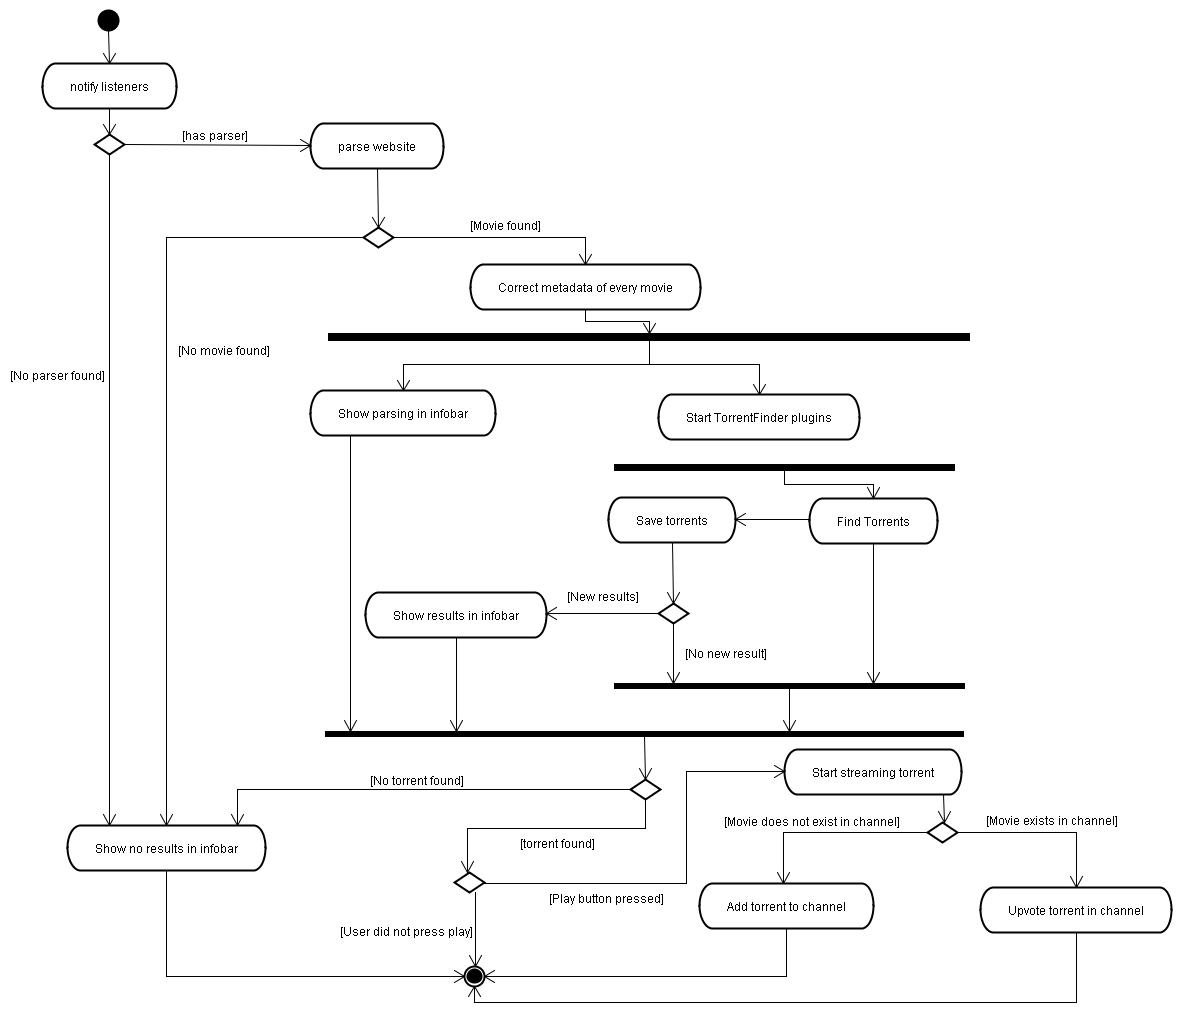
\includegraphics[width=0.8\textwidth]{TUPT-activitydiagram.jpg}
  \caption{Activity diagram of general TUPT functionality}
  \label{fig:activitytupt}
\end{figure}

\begin{figure}[hp]
  \centering
\tikzimgGeneralTUPT
  \caption{Class diagram for the entire TUPT package}
  \label{fig:classdiagramgeneraltupt}
\end{figure}

\begin{figure}[hp]
  \centering
\tikzimgSpecificTUPT
  \caption{Class diagram for the top-level TUPT package}
  \label{fig:classdiagramspecifictupt}
\end{figure}

\begin{figure}[hp]
  \centering
\tikzimgParser
  \caption{Class diagram for the Parser sub-package}
  \label{fig:classdiagramparser}
\end{figure}

\begin{figure}[hp]
  \centering
      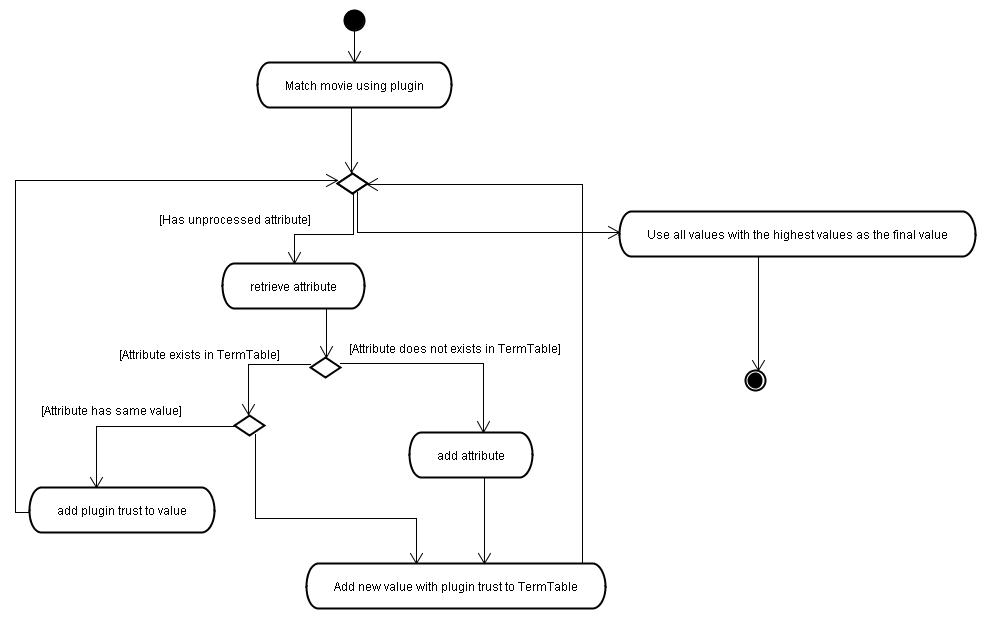
\includegraphics[width=0.8\textwidth]{Matcher-activitydiagram.jpg}
  \caption{Activity diagram of the Matcher sub-package}
  \label{fig:activitymatcher}
\end{figure}

\begin{figure}[hp]
  \centering
\tikzimgMatcher
  \caption{Class diagram for the Matcher sub-package}
  \label{fig:classdiagrammatcher}
\end{figure}

\begin{figure}[hp]
  \centering
      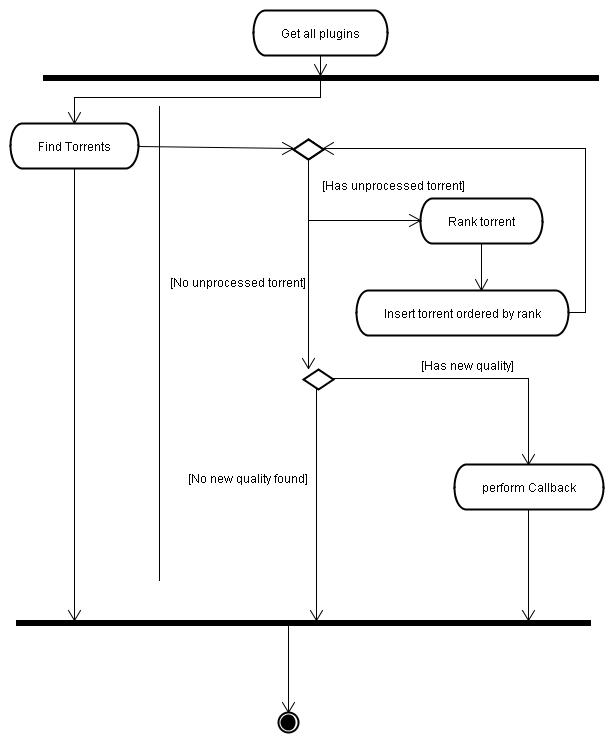
\includegraphics[width=0.8\textwidth]{TorrentFinder-activitydiagram.jpg}
  \caption{Activity diagram of the TorrentFinder sub-package}
  \label{fig:activitytorrentfinder}
\end{figure}

\begin{figure}[hp]
  \centering
\tikzimgTorrentFinder
  \caption{Class diagram for the TorrentFinder sub-package}
  \label{fig:classdiagramtorrentfinder}
\end{figure}

\begin{figure}[hp]
  \centering
\tikzimgChannels
  \caption{Class diagram for the Channels sub-package}
  \label{fig:classdiagramchannels}
\end{figure}

\section{Tests}
This is a section about tests: TODO

\end{document}
